\section{Neural Networks}
\subsection{Task 3: Theory}

\subsubsection*{a)}
The binary operation XOR, or exclusive or, cannot be represented by a single-layer neural network. If we look at the two binary input values as the two digits of a binary number, we get the range $[0, 3]$. Then applying the XOR function for this range, we get $[0, 1, 1, 0]$, which obviously cannot be represented by a linear function. 

\subsubsection*{b)}
A hyperparameter is a parameter which is set before, and not changed by, the learning process. Batch size and learning rate are examples of hyperparameters. 

\subsubsection*{c)}
The softmax function is a smooth approximation of the arg max function. The values being applied to the are shifted into the range $[0, 1]$, so that they can be interpreted as probabilities, and further as a probability density function, where the sum of the result is 1. 

\subsubsection*{d)}
\begin{equation}
    \label{eq:cost_function}
    C(y_n, \hat{y}_n) = (y_n - \hat{y}_n)^2, \hat{y}_n = 1
\end{equation}

Using \cref{eq:cost_function}, we calculate: 
\begin{align*}
        w_1' = \frac{ \partial C}{\partial w_1} 
    &= \frac{\partial C}{\partial y} \frac{\partial y}{\partial c_1} 
    \frac{\partial c_1}{\partial a_1} \frac{\partial a_1}{\partial w_1}
    = 2 * (y_n - \hat{y}_n) * 1 * 1 * w_1 = - 2 * (y_n - 1) \\
        w_2' = \frac{\partial C}{\partial w_2} 
    &= \frac{\partial C}{\partial y} \frac{\partial y}{\partial c_1} 
    \frac{\partial c_1}{\partial a_2} \frac{\partial a_2}{\partial w_2}
    = 2 * (y_n - \hat{y}_n) * 1 * 1 * w_2 = 2 * (y_n - 1) \\
        w_3' = \frac{\partial C}{\partial w_3} 
    &= \frac{\partial C}{\partial y} \frac{\partial y}{\partial c_2} 
    \frac{\partial c_2}{\partial a_3} \frac{\partial a_3}{\partial w_3}
    = 2 * (y_n - \hat{y}_n) * 1 * 1 * w_3 = - 2 * (y_n - 1) \\
        w_4' = \frac{\partial C}{\partial w_4} 
    &= \frac{\partial C}{\partial y} \frac{\partial y}{\partial c_2} 
    \frac{\partial c_2}{\partial a_4} \frac{\partial a_4}{\partial w_4}
    = 2 * (y_n - \hat{y}_n) * 1 * 1 * w_4 = - 4 * (y_n - 1) \\
        b_1' = \frac{\partial C}{\partial b_1} 
    &= \frac{\partial C}{\partial y} \frac{\partial y}{\partial c_1} 
    \frac{\partial c_1}{\partial b_1} 
    = 2 * (y_n - \hat{y}_n) * 1 * 1 = 2 * (y_n - 1) \\ 
        b_2' = \frac{\partial C}{\partial b_2}
    &= \frac{\partial C}{\partial y} \frac{\partial y}{\partial c_2} 
    \frac{\partial c_2}{\partial b_2} 
    = 2 * (y_n - \hat{y}_n) * 1 * 1 = 2 * (y_n - 1) 
\end{align*}

\subsubsection*{e)}
Calculating the current value for $y$: 
\begin{align*}
    a_1 &= 1,& a_2 &= 0,& a_3 &= 1,& a_4 &= -4 \\
    c_1 &= 2,& c_2 &= -4,& y_n  &= max(c_1, c_2) = 2
\end{align*}

\begin{equation}
    \label{eq:gradient_descent}
    \theta_{t+1} = w_t - \alpha \frac{\partial C}{\partial \theta_t}
\end{equation}

Using \cref{eq:gradient_descent} and $\alpha = 0.1$, we get: 
\begin{align*}
    w_{1, t + 1} 
    &= w_{1, t} - \alpha \frac{ \partial C}{\partial w_1} 
     = -1 - 0.1 * ( - 2 * (2 - 1)) = - 0.8 \\
    w_{3, t + 1} 
    &= w_{3, t} - \alpha \frac{ \partial C}{\partial w_3} 
     = -1 - 0.1 * (- 2 * (2 - 1)) = - 0.8 \\
    b_{1, t + 1} 
    &= b_{1, t} - \alpha \frac{ \partial C}{\partial b_1} 
     = 1 - 0.1 * 2 * (2 - 1) = 0.8
\end{align*}

\newpage
\subsection{Task 4: Programming}
\subsubsection*{a)}
The original training loss can be seen \cref{fig:training_loss} and the normalized here: \cref{fig:normalized_training_loss}. We may note that the loss converges quicker, and to a smaller value than the non-normalized data. This is as expected. 

We may note that it seems like certain of the validation images were too different to the training images to be classified, which manifests as a spike in the test-loss of the normalized figures. I think this is the reason, but I'm not quiet sure, and would like some pointers if there are any specifics. It is interesting that this problem only manifests when using the single-layered neural network with the normalized images. If the images were not normalized, or the neural network had a hidden layer, this problem disappeared. 

\begin{figure}[]
    \centering
    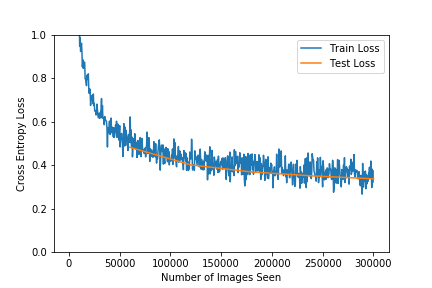
\includegraphics[width=1.00\textwidth]{figures/training/original_training_loss.png}
    \caption{Training and test loss before the task}
    \label{fig:training_loss}
\end{figure}

\begin{figure}[]
    \centering
    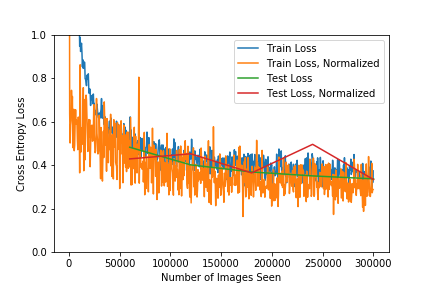
\includegraphics[width=1.00\textwidth]{figures/training/original_vs_normalized_training_loss.png}
    \caption{Original vs. normalized training and test loss}
    \label{fig:normalized_training_loss}
\end{figure}

\subsubsection*{b)}
For each class, the gray-scale images were generated by normalizing the weights for each class and reshaping the weights inverse of the way we convert an image to the input layer. We can see the weight image in the figures: \cref{fig:class_weight_0}, \cref{fig:class_weight_1}, \cref{fig:class_weight_2}, \cref{fig:class_weight_3}, \cref{fig:class_weight_4}, \cref{fig:class_weight_5}, \cref{fig:class_weight_6}, \cref{fig:class_weight_7}, \cref{fig:class_weight_8} and \cref{fig:class_weight_9}.  

This weights give what points of the image should increase the probability of that specific class being the correct one. As we only have one layer, this is a mapping of the input image to the output, and we can see the shapes that are \textit{extracted} by the weights, and we can note that they are similar to the number we are looking for. This can be especially well from \cref{fig:class_weight_0}, with the large negative space in the center being important to determining if a number is zero or not. 

\begin{figure}[]
    \centering
    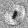
\includegraphics[width=0.50\textwidth]{figures/weights/class_0_weight_image.jpg}
    \caption{Class weight 0}
    \label{fig:class_weight_0}
\end{figure}

\begin{figure}[]
    \centering
    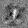
\includegraphics[width=0.50\textwidth]{figures/weights/class_1_weight_image.jpg}
    \caption{Class weight 1}
    \label{fig:class_weight_1}
\end{figure}

\begin{figure}[]
    \centering
    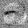
\includegraphics[width=0.50\textwidth]{figures/weights/class_2_weight_image.jpg}
    \caption{Class weight 2}
    \label{fig:class_weight_2}
\end{figure}

\begin{figure}[]
    \centering
    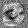
\includegraphics[width=0.50\textwidth]{figures/weights/class_3_weight_image.jpg}
    \caption{Class weight 3}
    \label{fig:class_weight_3}
\end{figure}

\begin{figure}[]
    \centering
    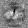
\includegraphics[width=0.50\textwidth]{figures/weights/class_4_weight_image.jpg}
    \caption{Class weight 4}
    \label{fig:class_weight_4}
\end{figure}

\begin{figure}[]
    \centering
    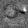
\includegraphics[width=0.50\textwidth]{figures/weights/class_5_weight_image.jpg}
    \caption{Class weight 5}
    \label{fig:class_weight_5}
\end{figure}

\begin{figure}[]
    \centering
    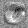
\includegraphics[width=0.50\textwidth]{figures/weights/class_6_weight_image.jpg}
    \caption{Class weight 6}
    \label{fig:class_weight_6}
\end{figure}

\begin{figure}[]
    \centering
    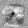
\includegraphics[width=0.50\textwidth]{figures/weights/class_7_weight_image.jpg}
    \caption{Class weight 7}
    \label{fig:class_weight_7}
\end{figure}

\begin{figure}[]
    \centering
    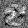
\includegraphics[width=0.50\textwidth]{figures/weights/class_8_weight_image.jpg}
    \caption{Class weight 8}
    \label{fig:class_weight_8}
\end{figure}

\begin{figure}[]
    \centering
    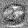
\includegraphics[width=0.50\textwidth]{figures/weights/class_9_weight_image.jpg}
    \caption{Class weight 9}
    \label{fig:class_weight_9}
\end{figure}

\subsubsection*{c)}
The accuracy is now way worse, as could be expected. This is due to the large learning rate. Even though a larger learning rate may give faster learning, it is also makes the gradient descent be less accurate, and we will not reach the correct weights to minimize the cost function. See \cref{fig:training_loss_learning_rate_1} for the cross entropy loss, but note that the plot does initially start even higher on the y-axis, but limiting it to 100 was done to show the shape of the function better. 

\begin{figure}[]
    \centering
    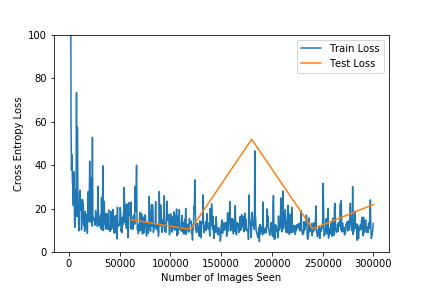
\includegraphics[width=1.00\textwidth]{figures/training/bad_learning_rate_training_loss.png}
    \caption{Training and test loss with learning rate 1}
    \label{fig:training_loss_learning_rate_1}
\end{figure}

\subsubsection*{d)}
From \cref{fig:training_loss_hidden_layer} we can see that the training loss and test loss end up converging faster to a lower cross entropy loss than the original neural network of \cref{fig:training_loss} and \cref{fig:normalized_training_loss}. This means that using the hidden layer both helps the neural network learn faster (using the same hyperparameters), as well as converge to a lower value, and the network is therefore both faster (to teach) and better (more likely to get the answer correct) than the original network. 

\begin{figure}[]
    \centering
    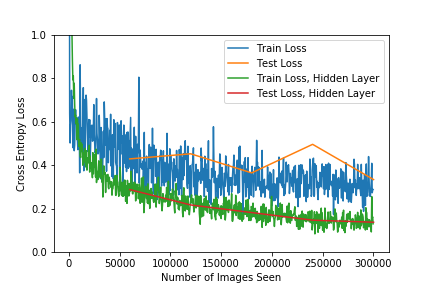
\includegraphics[width=1.00\textwidth]{figures/training/normalized_vs_hidden_layer_training_loss.png}
    \caption{Training and test loss with new hidden layer}
    \label{fig:training_loss_hidden_layer}
\end{figure}
